\documentclass{documentation}
\usepackage{tikz}
\usetikzlibrary{shapes.geometric, arrows}
\tikzstyle{module} = [rectangle, rounded corners, minimum width=3cm, minimum height=1cm,text centered, draw=black]
\tikzstyle{}

\title{Dokumentacja Techniczna Backend}

\author{Tomasz Chady}

\begin{document}

\maketitle

\tableofcontents

\section{Dokumentacja API}

\subsection{Endpointy}

\subsubsection{Logowanie}

Poniżej znajdują się endpointy odpowiedzialne za logowanie.
W odróżnieniu od innych endpointów, nie wymagają one autoryzacji.

\begin{itemize}
    \item POST /api/login
    \item POST /api/login-step2
\end{itemize}

\subsubsection{Użytkownicy}

Poniżej znajdują się endpointy odpowiedzialne za zarządzanie użytkownikami.

\begin{itemize}
    \item GET /api/profile
    \item POST /api/disable-2fa
    \item POST /api/generate-2fa-secret
    \item POST /api/verify-otp
\end{itemize}

\subsubsection{Administracja}

Poniżej wymienione są endpointy, powiązane z administracją systemem.
Z reguły posiadają swoje własne metody autoryzacji.

\begin{itemize}
    \item POST /api/signup
\end{itemize}

\subsection{Autoryzacja}

\section{Architektura Backendu}

\begin{figure}[h]
    \centering
    \begin{tikzpicture}[node distance=2cm]
        \node[module, fill=green!30, minimum width=10cm] (index) {index.js};

        \node[module, fill=orange!30, below of=index, xshift=-2cm, minimum width=6cm] (jwt) {jwt};
    \end{tikzpicture}
    \caption{Schemat API\label{fig:API}}
\end{figure}

\begin{figure}[h]
    \centering
    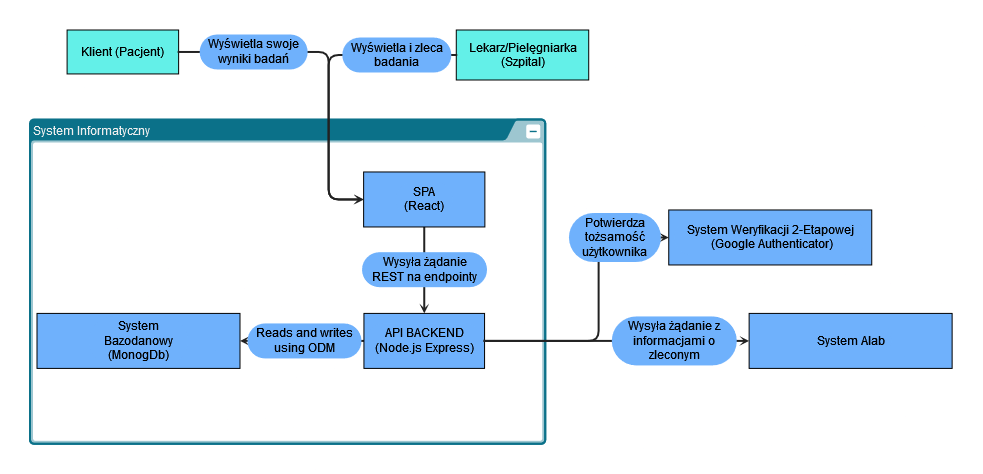
\includegraphics[width=0.8\textwidth]{Level_2_C4_Model.png}
    \caption{Schemat architektury\label{fig:arch}}
\end{figure}

\begin{figure}[h]
    \centering
    \begin{tikzpicture}[node distance=3cm]
        \node[module, fill=green!30] (index) {index.js};

        \node[module, fill=orange!30, below of=index, xshift=-6cm] (db) {db.js};
        \node[module, fill=blue!30, below of=db] (models) {models.js};
        
        \node[module, fill=red!30, below of=index, xshift=0] (controllers) {controllers.js};

        \node[module, fill=yellow!30, below of=index, xshift=6cm] (auth) {auth.js};
        \node[module, fill=red!60, below of=auth] (env) {env.js};

        
        \draw [->] (db) -- (index);
        \draw [->] (controllers) -- (index);
        \draw [->] (auth) -- (index);
        \draw [dashed, ->] (auth) -- node[anchor=center]{Passport.js} (controllers);
        \draw [->] (env) -- (auth);
        \draw [->] (env) -- (controllers);
        \draw [->] (models) -- (db);
        \draw [->] (models) -- (auth);
        \draw [->] (models) -- (controllers);

    \end{tikzpicture}
    \caption{Schemat wymagań\label{fig:dependency}}
\end{figure}

\section{Baza danych}

\subsection{Schemat}

\subsection{Modele}

\end{document}